Next, we evaluate the models’ ability to predict the bees’ orientation angles based on the predicted head and tail masks.
\Cref{tab:orientation_results} summarizes the orientation error on the test set, reported as the mean, median and key percentiles.

ResUNet18 achieves slightly better orientation accuracy than UNet3: the mean error is reduced from \qty{14.8}{\degree} to \qty{13.2}{\degree}, and the median error from \qty{6.5}{\degree} to \qty{5.7}{\degree}.
However, both models remain well above the baseline error of approximately \qty{0.25}{\degree} measured between the ground-truth masks and the ground-truth CSV angles.
This suggests that imperfect segmentations rather than annotation noise are the main limiting factor.

\Cref{fig:orientation_error_hist_cdf} shows the distribution of absolute orientation errors for each model, presented as both a histogram and a CDF.
Both models exhibit a strong concentration of predictions with errors below \qty{20}{\degree}, with ResUNet18 producing slightly more low-error predictions than UNet3.
The overall distributions are otherwise similar, with both models displaying a noticeable secondary peak at very high errors (approximately \qty{180}{\degree}), which is likely caused by head–tail confusion or annotation errors.
We investigate this phenomenon further in \cref{subsec:qualitative-analysis}.

We also examined the signed orientation errors to check for systematic directional bias in the predictions (see \Cref{fig:appendix_unet3_orientation,fig:appendix_resunet18_orientation}).
No substantial bias was observed, with the errors being approximately symmetrically distributed around zero.


\begin{table}[htbp]
    \centering
    \caption{Absolute orientation error against ground‑truth CSV angles.}
    \label{tab:orientation_results}
    \begin{tabular}{lcccccc}
        \toprule
        \textbf{Model} & \textbf{Mean $\pm$ SD}                          & \textbf{Median}     & \textbf{75\%ile}     & \textbf{90\%ile} & \textbf{95\%ile} & \textbf{99\%ile} \\
        \midrule
        UNet3          & \qty{14.79}{\degree} $\pm$ \qty{31.57}{\degree} & \qty{6.49}{\degree} & \qty{12.16}{\degree}   & \qty{21.91}{\degree}   & \qty{50.57}{\degree}   & \qty{174.60}{\degree}  \\
        ResUNet18      & \qty{13.23}{\degree} $\pm$ \qty{31.12}{\degree} & \qty{5.73}{\degree} & \qty{10.59}{\degree}   & \qty{17.98}{\degree}   & \qty{30.25}{\degree}   & \qty{175.74}{\degree}  \\
        \bottomrule
    \end{tabular}
\end{table}

\begin{figure}[htbp]
    \centering
    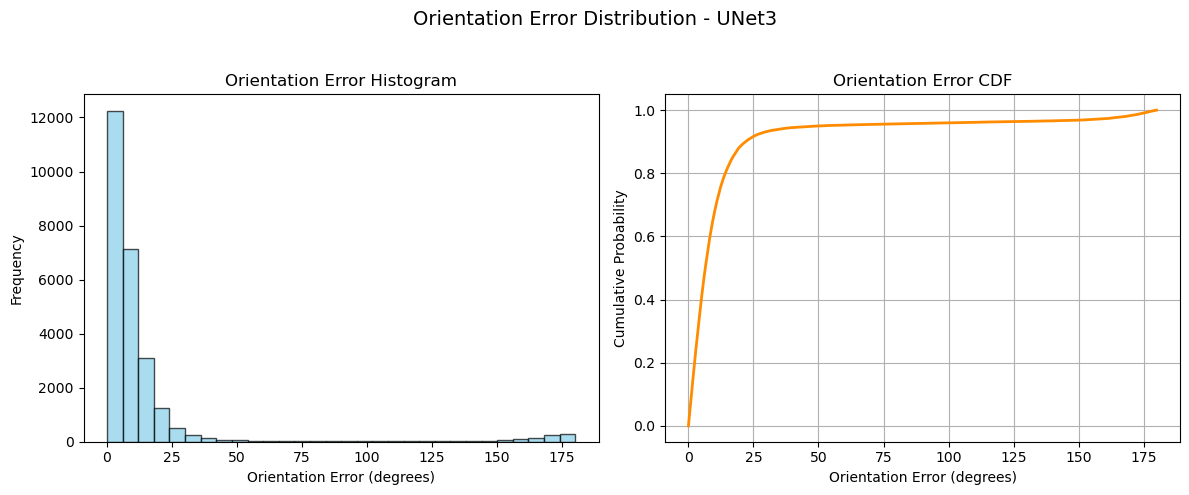
\includegraphics[width=\textwidth]{figures/results/3 - orientation estimation/UNet3 Orientation Error.png}

    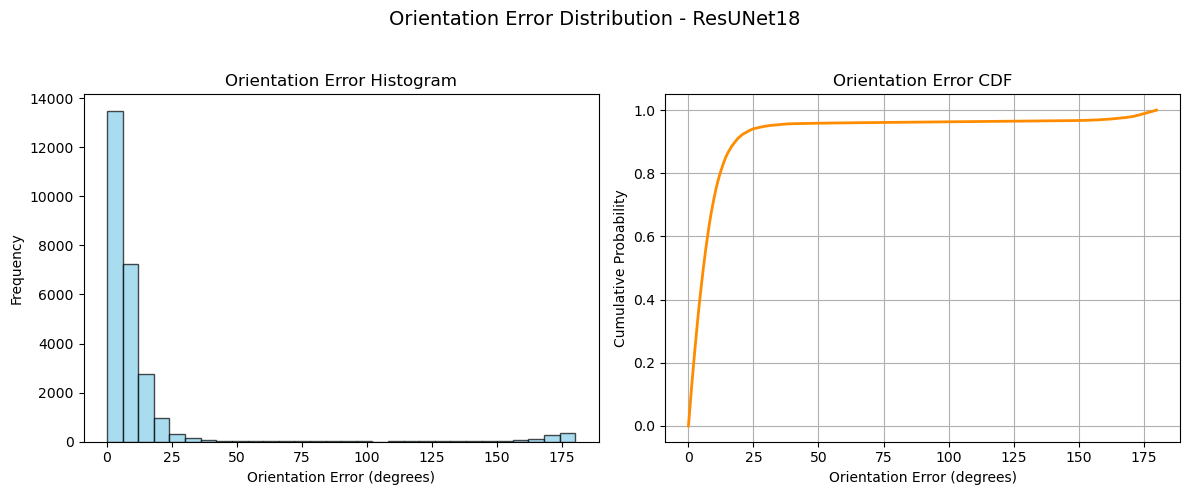
\includegraphics[width=\textwidth]{figures/results/3 - orientation estimation/ResUNet18 Orientation Error.png}
    \caption{
        Orientation error distribution on the test set for UNet3 (\textbf{top}) and ResUNet18 (\textbf{bottom}).
        For each model, the left panel shows a histogram of absolute orientation errors; the right panel shows the cumulative distribution function (CDF).
        Both models produce similar distributions with most errors below \qty{20}{\degree} and a small bump at very high errors ($\approx$\qty{180}{\degree}).
    }
    \label{fig:orientation_error_hist_cdf}
\end{figure}